\section{Practice: Wireless doorbell}\label{pract:wirelessDoorbell}

This practice guides you through the construction of a wireless doorbell system. It is composed by two components: the switch and the buzzer.

On the switch side, we will be prototyping a layout like the one shown in Figure~\ref{fig:wirelessDoorbellSwitch}. While the sound will be produced by a buzzer on the other radio, like in Figure~\ref{fig:wirelessDoorbellBuzzer}.

You will need:

\begin{itemize}
  \item Eventhough the two components may fit in one breadboard; to make it more real, it is better to use two separate breadboards.
  \item Hookup wire. It is recommended to have at least four different colors.
  \item Two Arduino boards.
  \item USB A-to-B cable for the Arduinos.
  \item One $10$K resistor.
  \item One momentary switch or pushbutton for input.
  \item One buzzer for output.
  \item One XBee radio configured as \texttt{ZIGBEE COORDINATOR AT}.
  \item One XBee radio configured as \texttt{ZIGBEE ROUTER AT}.
  \item Two breakout boards.
  \item USB cable for the XBee breakout board.
\end{itemize}

Every ZigBee network has only one coordinator. Other nodes can be configured as routers. To configure your XBee radios, please refer to Chapter~\ref{xbeeRoleConfiguration}.

It is strongly suggested that you mark down the XBees to distinguish the coordinator from the router(s).

\subsection{Wireless doorbell connections layout}

\subsubsection{Switch}
Follow these guidelines to prepare the connections for the switch that will make the doorbell ring (or buzz in our case). If lost, you can always take a look at the final layout in Figure~\ref{fig:wirelessDoorbellSwitch}.

\begin{enumerate}
  \item Energize the breadboard by hooking up a {\color{red}{red}} wire from the Arduino $3.3$V output to one of the power rails of the breadboard.
  \item Hook up a {\color{blue}{blue}} wire from the ground (GND) connection on the Arduino to the ground rail on the breadboard.
  \item Place the XBee/breakout board with both sides on different sections of the breadboard, in a way that the space separating the sections passes under the XBee/breakout board.
  \item Use a {\color{red}{red}} wire to connect pin $3.3$V (or pin $2$ as in Figure~\ref{fig:xbeeBreakoutBoardPins}) of the XBee to the power rail on the breadboard.
\end{enumerate}


\begin{figure}[htbp]
  \centering
  \includegraphics[width=\linewidth]{figures/doorbellSwitch.eps}
  \caption{Wireless doorbell: switch layout
  \label{fig:wirelessDoorbellSwitch}}
\end{figure}

\begin{figure}[htbp]
  \centering
  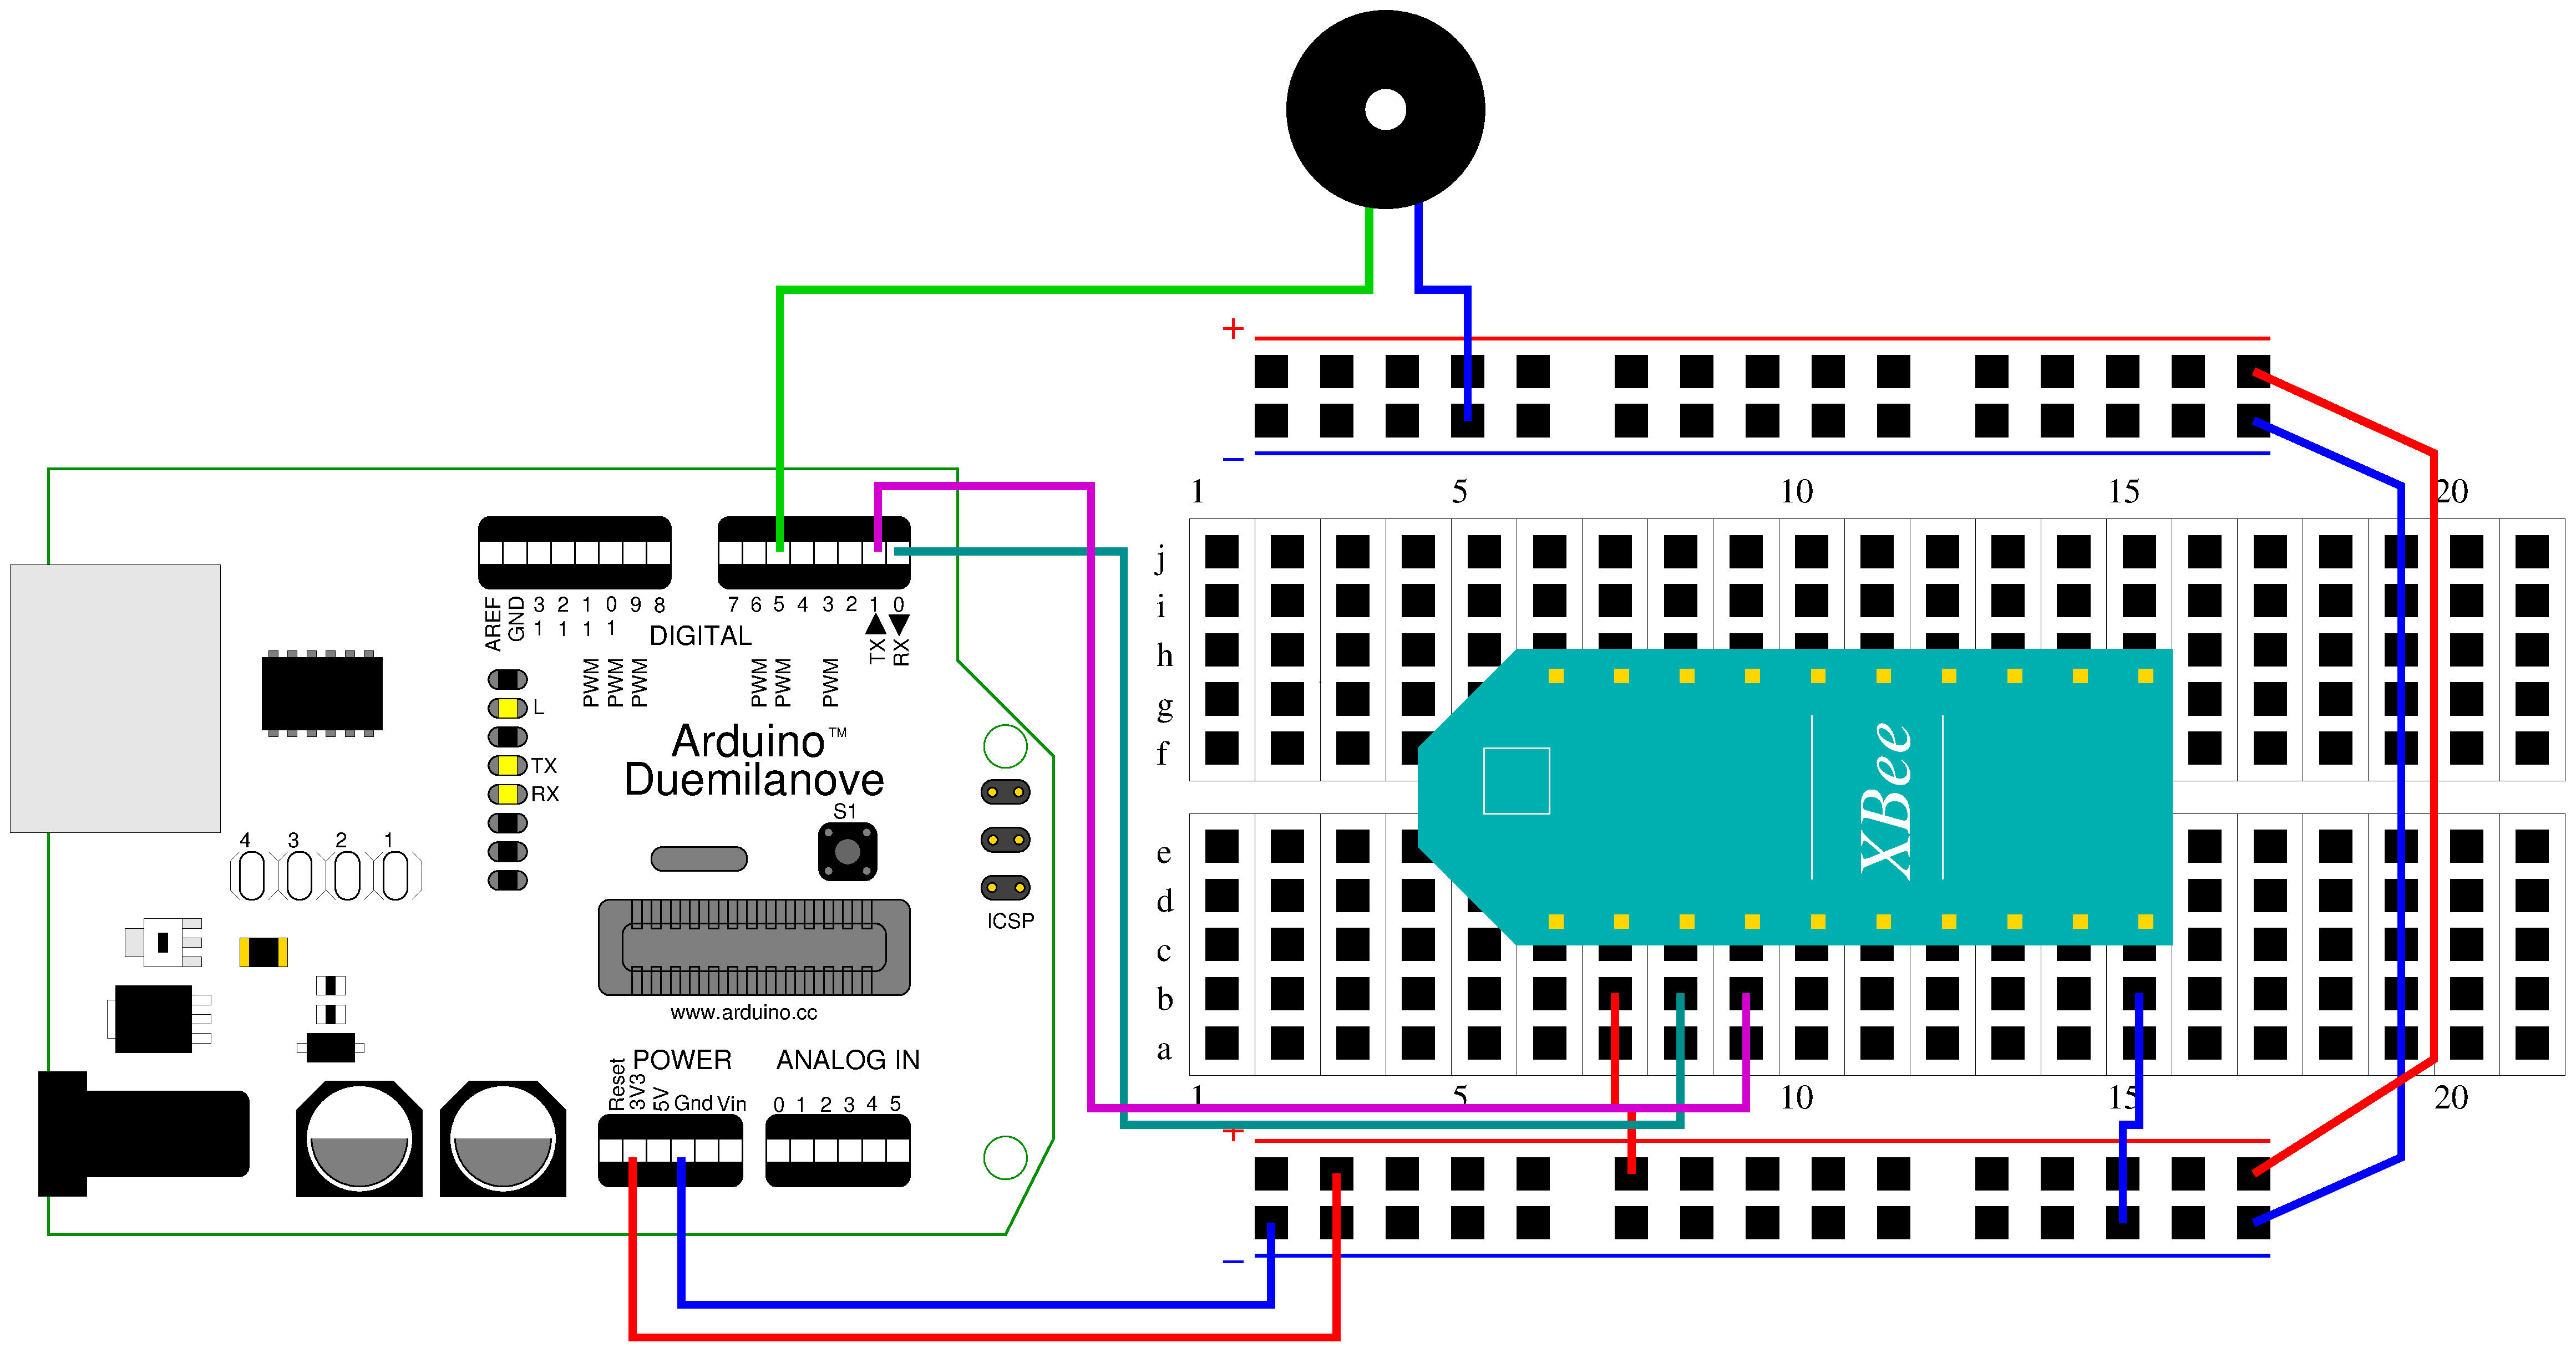
\includegraphics[width=\linewidth]{figures/doorbellBuzzer.eps}
  \caption{Wireless doorbell: buzzer layout
  \label{fig:wirelessDoorbellBuzzer}}
\end{figure}